\documentclass[a4paper, twocolumn]{article}

%\setlength{\parskip}{0.5\baselineskip}
\usepackage{pdfpages}

\usepackage{geometry}
% \geometry{left = 2.54 cm, right = 2.54 cm, top = 2.54 cm, bottom = 2.54 cm}
\geometry{left = 1 cm, right = 1 cm, top = 1 cm, bottom = 1 cm}

\usepackage{setspace}
\renewcommand{\baselinestretch}{1.0}
\usepackage{indentfirst}
\setlength{\parindent}{2em}

%\usepackage{fontspec}
%\setmainfont{Times New Roman}

\usepackage{ulem}
\usepackage{graphicx}
%\usepackage{wrapfig}
\usepackage{enumerate}
\usepackage{xcolor}
\usepackage{subcaption}
\usepackage{float}
\usepackage{amsmath, amssymb, amsthm}
\usepackage{booktabs}

\pagestyle{empty} % Not showing page number

\begin{document}
\renewcommand{\thesection}{\Roman{section}}
\renewcommand{\thesubsection}{\Alph{subsection}}
\renewcommand{\thesubsubsection}{\thesubsection.\arabic{subsubsection}}
\renewcommand{\d}{\: \mathrm{d} }
\newcommand{\e}{\mathrm{e}}

\section{Chapter 10}
    \begin{figure}[H]
        \centering
        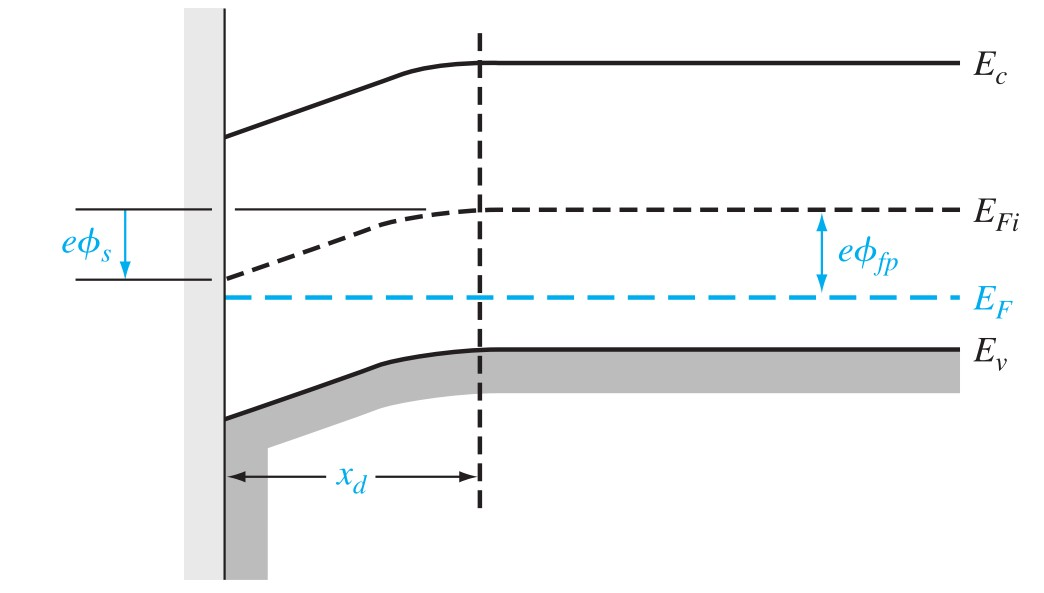
\includegraphics[width=0.9\linewidth]{Energy-band-diagram-PMOS-and-surface-potential.jpg}
        \label{fig:Energy-band-diagram-PMOS-and-surface-potential.jpg}
    \end{figure}
    \begin{equation*}
        \begin{aligned}
            \phi_{fp} &= V_t \ln \left( \frac{N_a}{n_i}  \right) \\
            x_d &= \left( \frac{2 \varepsilon_s \phi_s}{e N_a}  \right)^{1/2} 
        \end{aligned}
    \end{equation*}
    \begin{equation*}
        \boxed{x_{dT} = \left( \frac{4\varepsilon_s \phi_{fp} }{e N_a} \right)^{1/2}}
    \end{equation*}
    
    \begin{figure}[H]
        \centering
        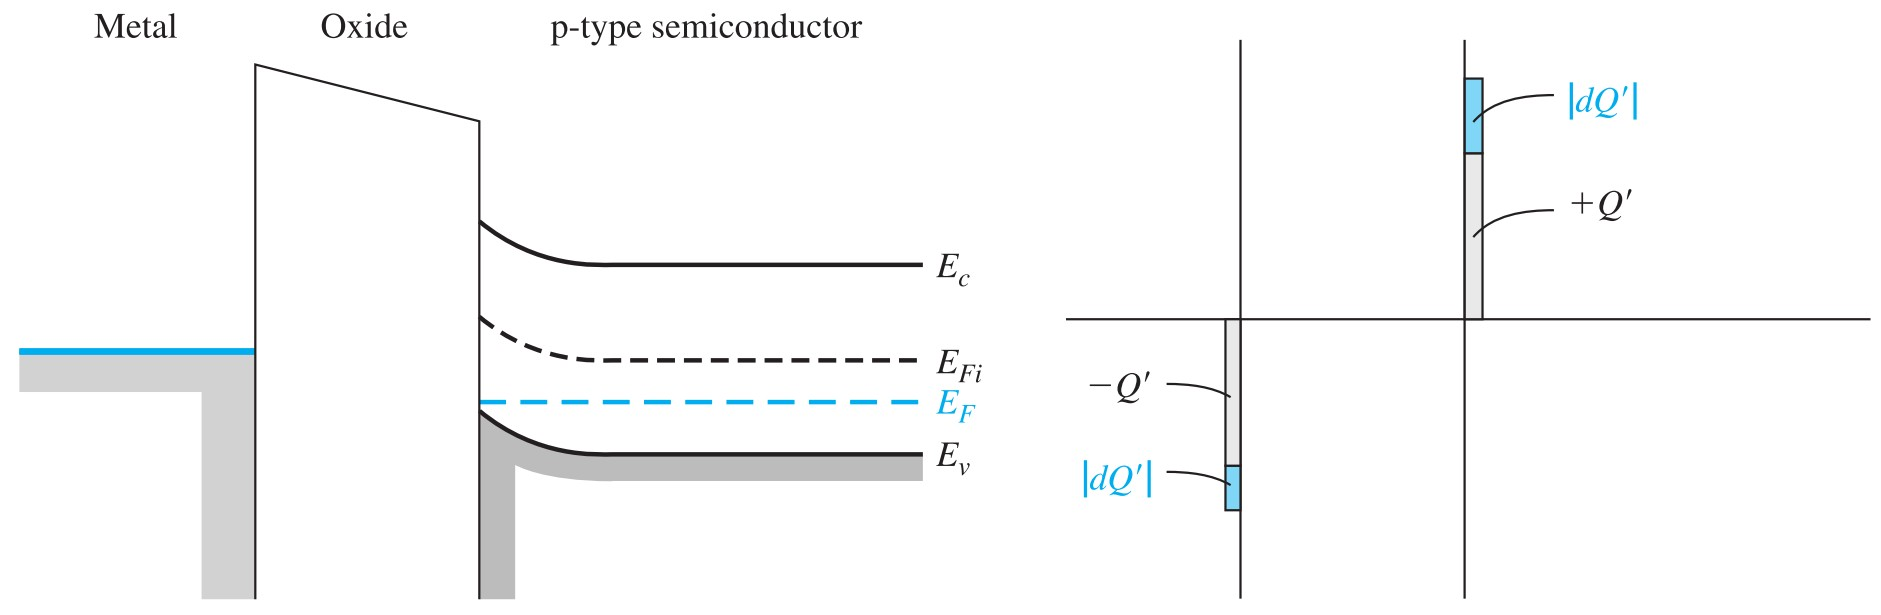
\includegraphics[width=0.9\linewidth]{C-V-accumulation.jpg}
        \label{fig:C-V-accumulation.jpg}
    \end{figure}
    \begin{equation*}
        C^\prime (\text{acc}) = C_{ox} = \frac{\varepsilon_{ox} }{t_{ox} }  
    \end{equation*}
    \begin{figure}[H]
        \centering
        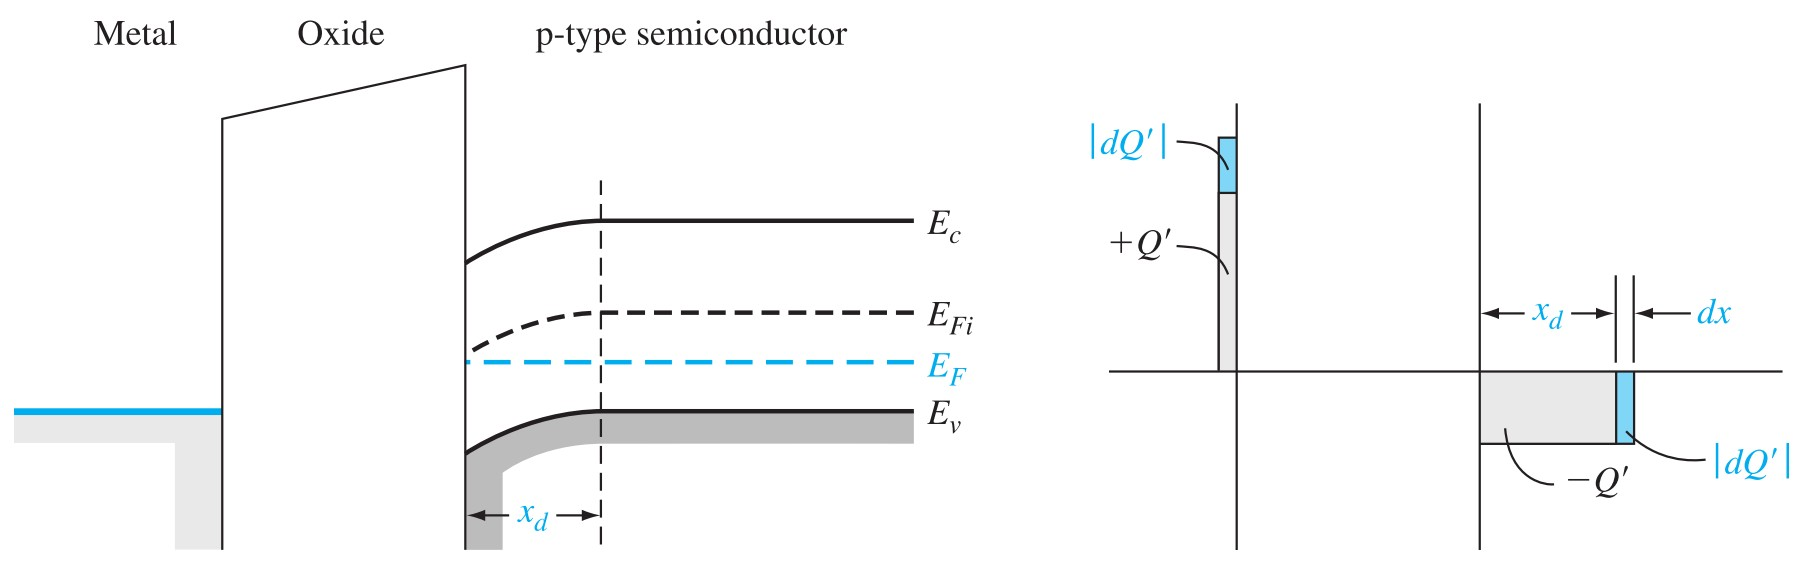
\includegraphics[width=0.9\linewidth]{C-V-depletion.jpg}
        \label{fig:C-V-depletion.jpg}
    \end{figure}
    \begin{equation*}
        \begin{aligned}
            C^\prime (\text{depl}) &= \frac{C_{ox} C^\prime_{SD} }{C_{ox} + C^\prime_{SD} } \\
            &= \frac{\varepsilon_{ox} }{t_{ox} + \left( \frac{\varepsilon_{ox} }{\varepsilon_s}  \right)x_d } 
        \end{aligned}
    \end{equation*}
    \begin{equation*}
        C^\prime_{min} = \frac{\varepsilon_{ox} }{t_{ox} + \left( \frac{\varepsilon_{ox} }{\varepsilon_s}  \right) x_{dT} } 
    \end{equation*}
    \begin{figure}[H]
        \centering
        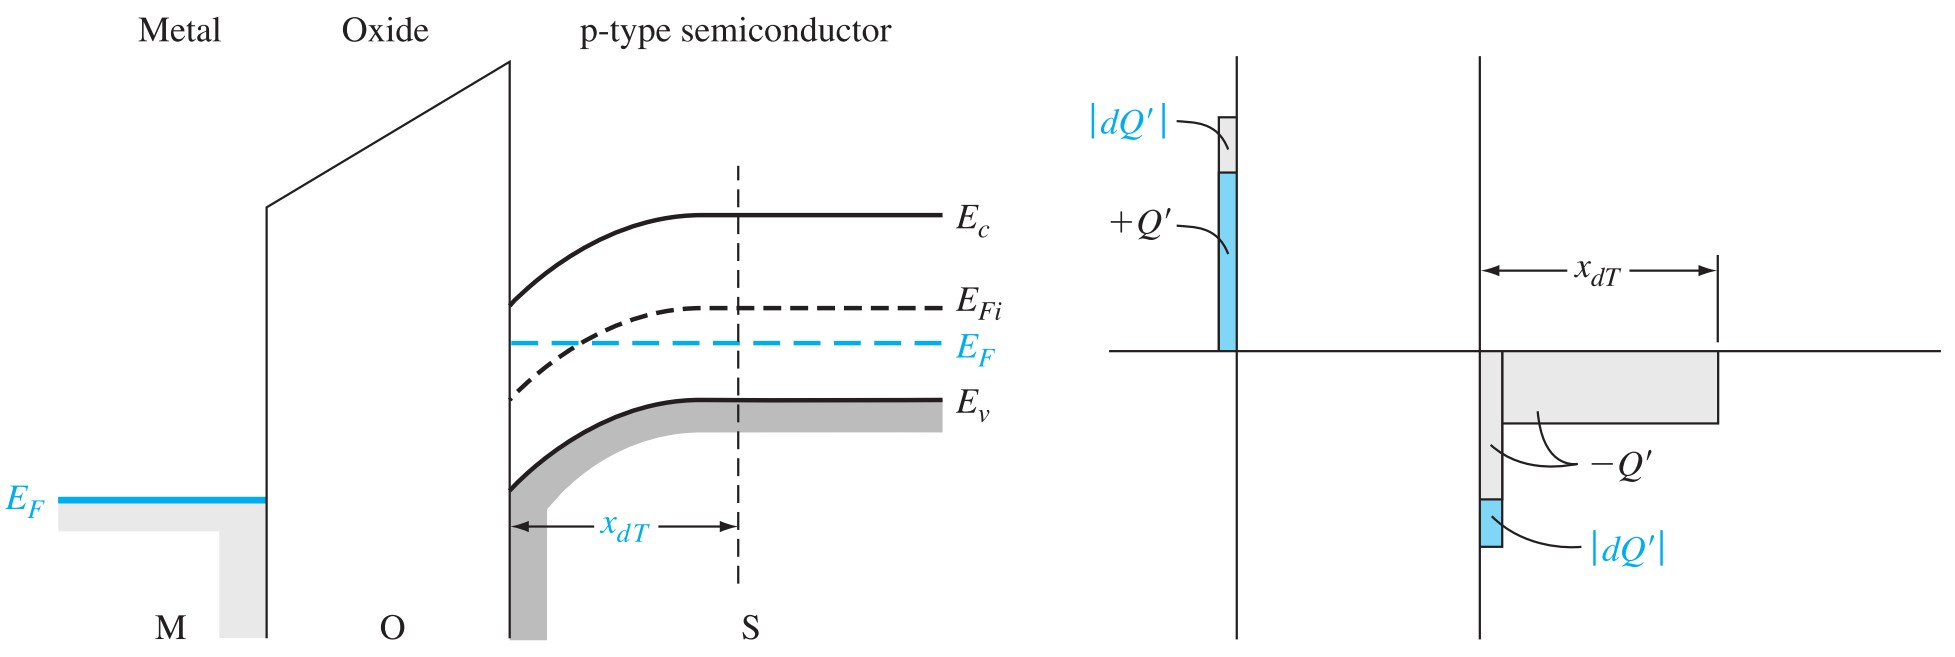
\includegraphics[width=0.9\linewidth]{C-V-inversion.jpg}
        \label{fig:C-V-inversion.jpg}
    \end{figure}
    \begin{equation*}
        C^\prime (\text{inv}) = C_{ox} = \frac{\varepsilon_{ox} }{t_{ox}}
    \end{equation*}
    \begin{figure}[H]
        \centering
        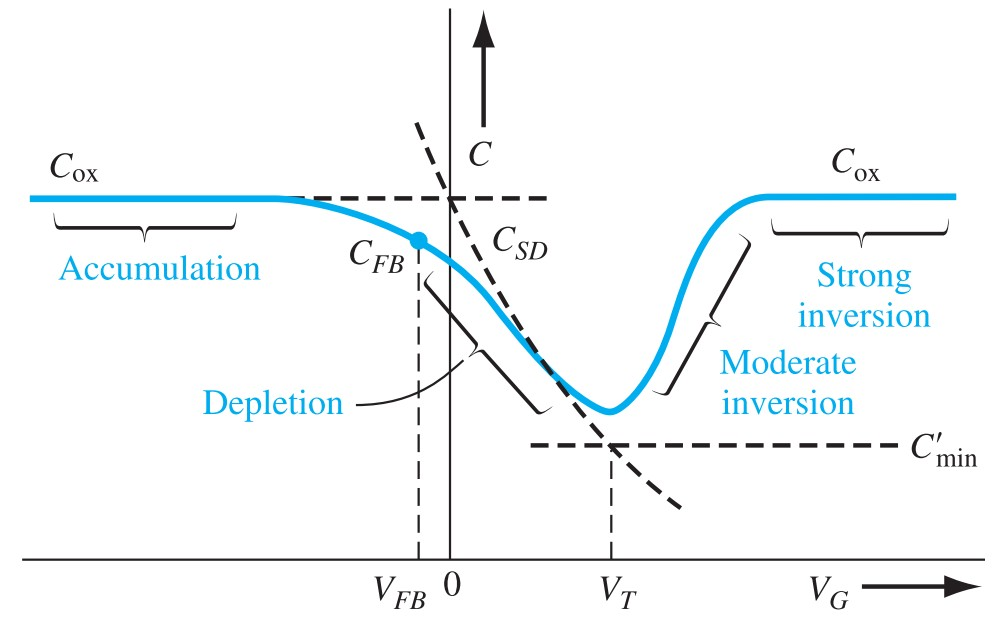
\includegraphics[width=0.8\linewidth]{C-V-graph-low-frequency.jpg}
        \label{fig:C-V-graph-low-frequency.jpg}
    \end{figure}
    \begin{equation*}
        \begin{aligned}
            C^\prime_{FB} = \frac{\varepsilon_{ox} }{t_{ox} + \left( \frac{\varepsilon_{ox} }{\varepsilon_s}  \right) \sqrt{\left( \frac{kT}{e}  \right) \left( \frac{\varepsilon_s}{eN_a}  \right)}} 
        \end{aligned}
    \end{equation*}
    \subsection*{Non-ideal Effects}
    \par 1. Frequency effects
    \begin{figure}[H]
        \centering
        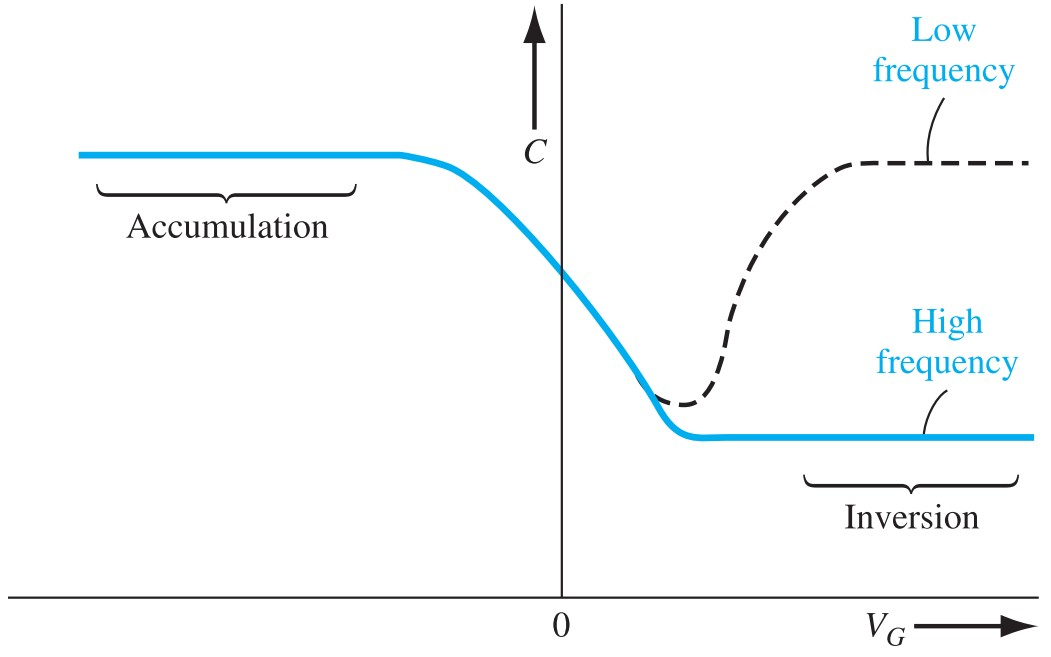
\includegraphics[width=0.6\linewidth]{Frequency-effect.jpg}
        \label{fig:Frequency-effect.jpg}
    \end{figure}
    \par 2. Work Function Difference
    \begin{figure}[H]
        \centering
        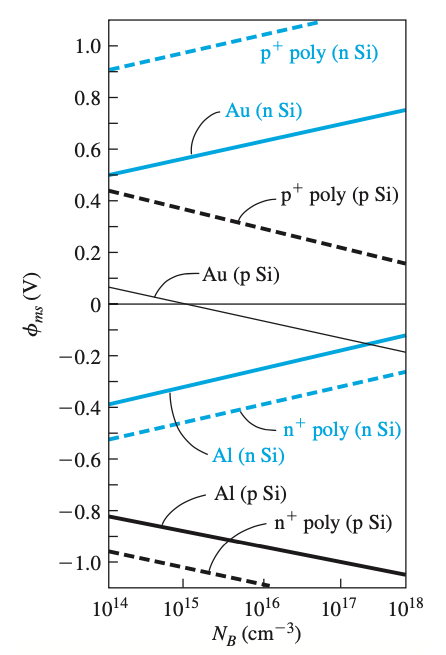
\includegraphics[width=0.6\linewidth]{Phi-ms.png}
    \end{figure}
    \par 3. Fixed Charge
    \par 4. Surface states
    \begin{figure}[H]
        \centering
        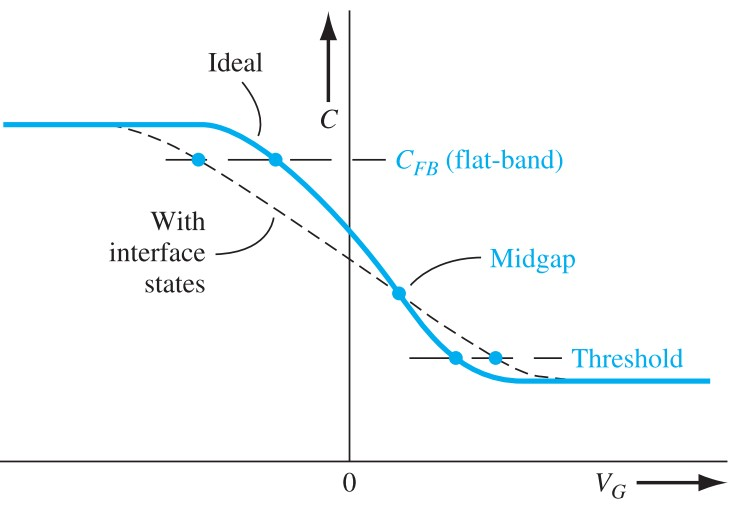
\includegraphics[width=0.6\linewidth]{Surface-states.jpg}
        \label{fig:Surface-states.jpg}
    \end{figure}
    
    \begin{equation*}
        \boxed{
        \begin{aligned}
            \left| Q^\prime_{SD} (\text{max}) \right| &= eN_a x_{dT} = 2 \sqrt{e \varepsilon_s N_a \phi_{fp} } \\
            V_{TN} &= \frac{\left| Q^\prime_{SD} (\text{max}) \right|}{C_{ox} } + V_{FB} + 2 \phi_{fp}  \\
            V_{TP} &= - \frac{\left| Q^\prime_{SD} (\text{max}) \right|}{C_{ox} } + V_{FB} - 2 \phi_{fn}  \\
            V_{FB} &= \phi_{ms} - \frac{Q^\prime_{ss} }{C_{ox}}\cdot \frac{x}{d} 
        \end{aligned}
        }
    \end{equation*}
    
    \begin{figure}[H]
        \centering
        \begin{subfigure}[t]{0.45\linewidth}
            \centering
            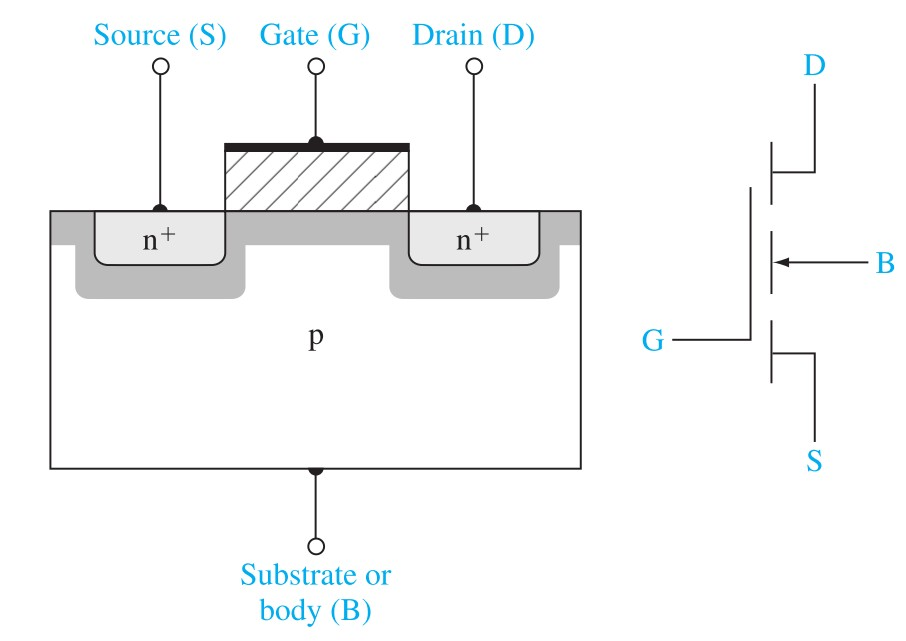
\includegraphics[width=0.9\linewidth]{NMOS-enhancement.jpg}
            \caption{n-channel enhancement MOSFET}
            \label{subfig:NMOS-enhancement.jpg}
        \end{subfigure}
        \begin{subfigure}[t]{0.45\linewidth}
            \centering
            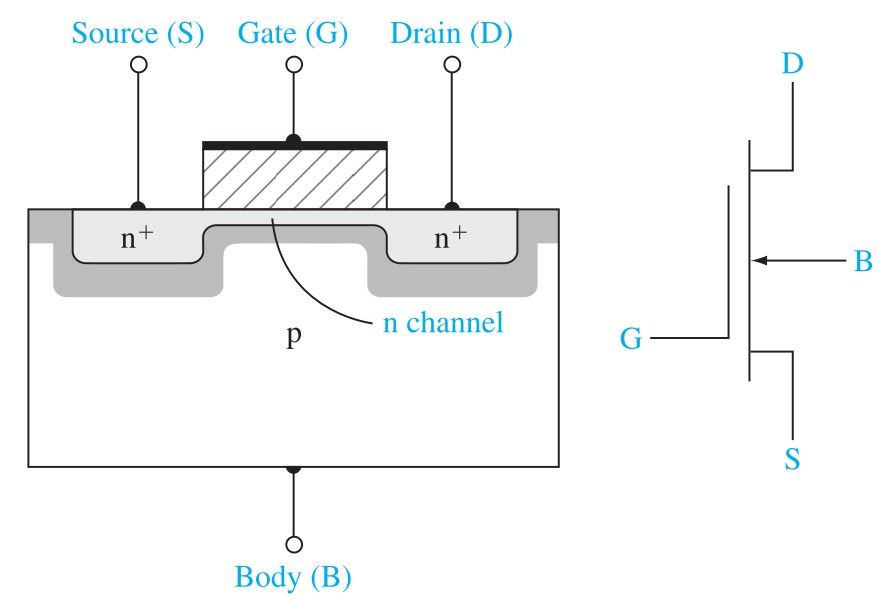
\includegraphics[width=0.9\linewidth]{NMOS-depletion.jpg}
            \caption{n-channel depletion MOSFET}
            \label{subfig:NMOS-depletion.jpg}
        \end{subfigure}
    \end{figure}
    \begin{figure}[H]
        \centering
        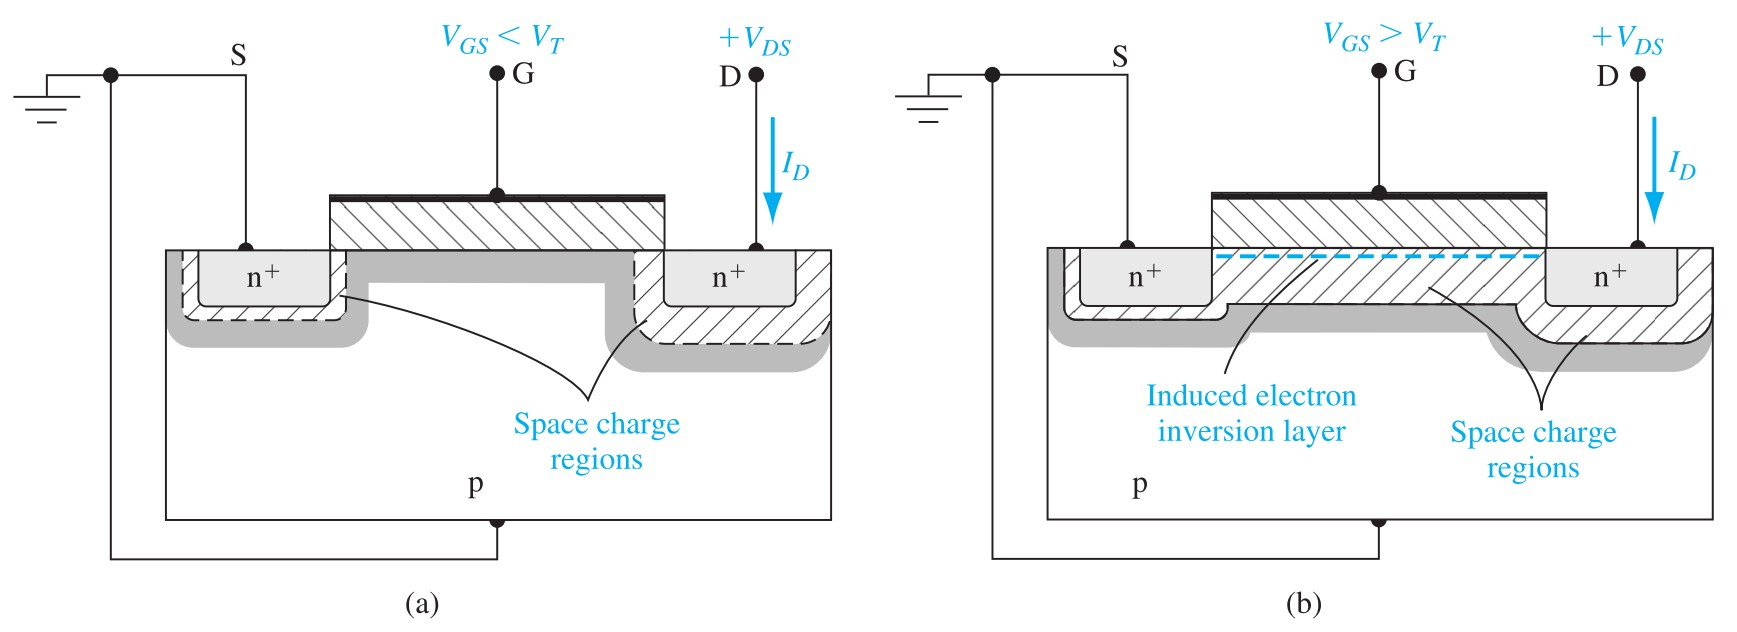
\includegraphics[width=0.9\linewidth]{Current-voltage-relationship.jpg}
        \caption{(a) $V_{GS} < V_T$, (b) $V_{GS} > V_T$}
        \label{fig:Current-voltage-relationship.jpg}
    \end{figure}
    \begin{itemize}
        \item $V_{DS} $ low ($V_{DS} < V_{GS} - V_T$): act as a controllable resistor.
        \begin{equation*}
            \begin{aligned}
                \boxed{I_D = \mu_n C_{ox} \frac{W}{L} \left( V_{GS}  - V_T - \frac{V_{DS}}{2}  \right) V_{DS}}
            \end{aligned}
        \end{equation*}
        \item $V_{DS}$ high ($V_{DS} \ge V_{GS} - V_T $): saturation
        \begin{equation*}
            \begin{aligned}
                \boxed{I_D = \mu_n C_{ox} \frac{W}{2L} \left( V_{GS} - V_T \right)^2 \quad (\text{saturation})}
            \end{aligned}
        \end{equation*}
    \end{itemize}
    \begin{equation*}
        \begin{aligned}
            g_{m} &= \frac{\partial I_D}{\partial V_{GS} } \\ 
            &= \left\{
                \begin{aligned}
                    & \mu_n C_{ox} \frac{W}{L} V_{DS} ,\qquad&& 0 < V_{DS} < V_{GS} - V_T \\
                    & \mu_n C_{ox} \frac{W}{L} \left( V_{GS}  - V_T \right) ,\qquad&& V_{DS} > V_{GS} - V_T
                \end{aligned}
            \right.
        \end{aligned}
    \end{equation*}
    \par Substrate Bias Effects:
    \begin{equation*}
        \boxed{
        \begin{aligned}
            \Delta V_T &= - \frac{\Delta Q^\prime_{SD} }{C_{ox} } = \frac{\sqrt{2 e \varepsilon_s N_a}}{C_{ox} }  \left[ \sqrt{2\phi_{fp} + V_{SB}  } - \sqrt{2 \phi_{fp}}\right] \\
            &= \gamma \left[ \sqrt{2\phi_{fp} + V_{SB}  } - \sqrt{2 \phi_{fp}}\right], \qquad \gamma = \frac{\sqrt{2 e \varepsilon_s N_a}}{C_{ox} }
        \end{aligned}
        }
    \end{equation*}
    
\section{Chapter 11}
    \par I - Subthreshold Conduction (Leakage Current) \\
        When $V_{GS} < V_T$, $I_D \propto \exp\left( \frac{qV_{GS} }{nkT}  \right)$
    \begin{equation*}
        S = n \left( \frac{kT}{q} \ln (10) \right) (\text{Volts per decade})
    \end{equation*}
    \par II - Channel Length Modulation \\
    \begin{figure}[H]
        \centering
        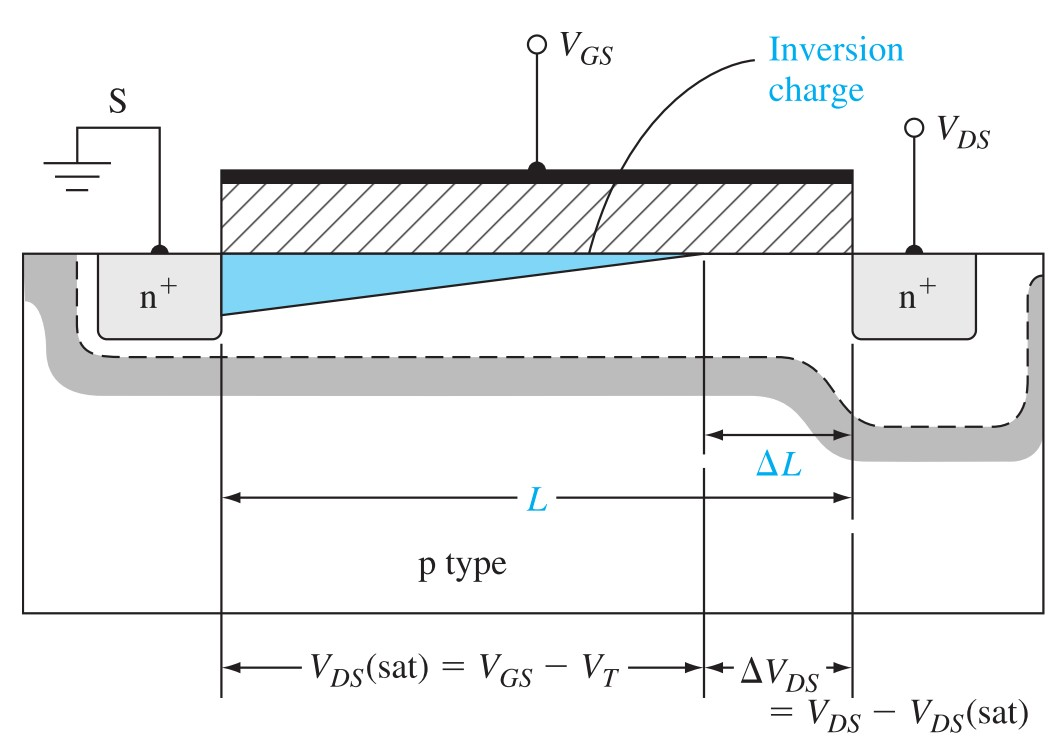
\includegraphics[width=0.9\linewidth]{Channel-length-modulation.jpg}
        \label{fig:Channel-length-modulation.jpg}
    \end{figure}
    \begin{equation*}
        \Delta L=\sqrt{\frac{2\epsilon_s}{eN_a}}\cdot[\sqrt{\phi_{fp}+V_{DS}(sat)+\Delta V_{DS}}-\sqrt{\phi_{fp}+V_{DS}(sat)}]
    \end{equation*}
    \begin{equation*}
        \begin{aligned}
             I^\prime_D &= \mu_n C_{ox} \frac{W}{2L} \left[\left( V_{GS} - V_T \right)^2  (1 + \lambda V_{DS}) \right] \\
            %  I^\prime_D &= \frac{L}{L - \Delta L} I_D
        \end{aligned}
    \end{equation*}
    \par III - Velocity Saturation \\
    \begin{equation*}
        \begin{aligned}
            I_{DSAT} &= WC_{ox} \left[ V_{GS} - V_{T} - \frac{V_{DSAT} }{2}  \right] v_{sat} \\
        \end{aligned}
    \end{equation*}
    where $V_{DSAT} = \frac{L}{\mu_n} v_{sat}$.
    \par IV - Short Channel Effect \\
    \begin{figure}[H]
        \centering
        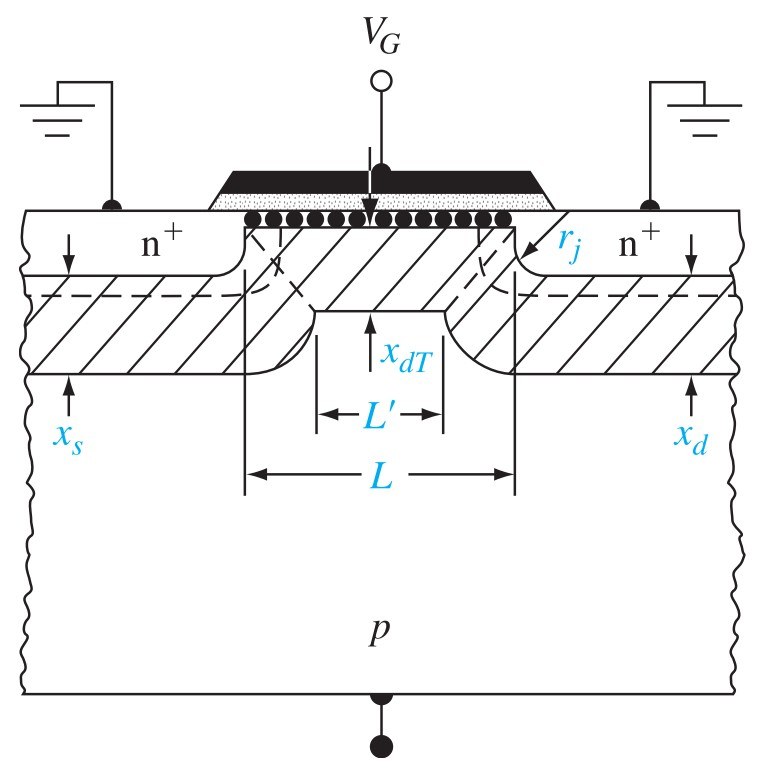
\includegraphics[width=0.5\linewidth]{Short-channel-effects.jpg}
        \label{fig:Short-channel-effects.jpg}
    \end{figure}   
    % \begin{equation*}
    %     \Delta V_T=-\frac{eN_ax_{dT}}{C_{ox}}[\frac{r_j}{L}(\sqrt{1+\frac{2x_{dT}}{r_j}}-1)]​​
    % \end{equation*}
    \par V - Narrow Channel Effect \\
    % \begin{equation*}
    %     \Delta V_T=\frac{eN_ax_{dT}}{C_{ox}}(\frac{\xi x_{dT}}{W})​
    % \end{equation*}
    
    \resizebox*{\linewidth}{!}{ %
        % \begin{equation*}
        $
            \begin{aligned}
                I_D = 
                \left\{
                    \begin{aligned}
                        & \sim \exp\left( \dfrac{eV_{GS} }{nkT} \left[ 1 - \exp\left( \dfrac{-e V_{DS} }{kT}  \right) \right]  \right) && V_{GS} - V_T < 0 \\
                        & \mu_n C_{ox} \dfrac{W}{2L} \left[\left( V_{GS} - V_T \right)^2  (1 + \lambda V_{DS}) \right] && 0 \le V_{GS} - V_T < V_{DS}  \\
                        & I_D = \mu_n C_{ox} \dfrac{W}{L} \left( V_{GS}  - V_T - \dfrac{V_{DS}}{2}  \right) V_{DS} && V_{DS} \le V_{GS} - V_T  \\
                    \end{aligned}
                \right.
            \end{aligned}
        $
        % \end{equation*}
    }
    \begin{equation*}
        k_n^\prime = \mu_n C_{ox} 
    \end{equation*} 
\section{Chapter 12}
    \begin{figure}[H]
        \centering
        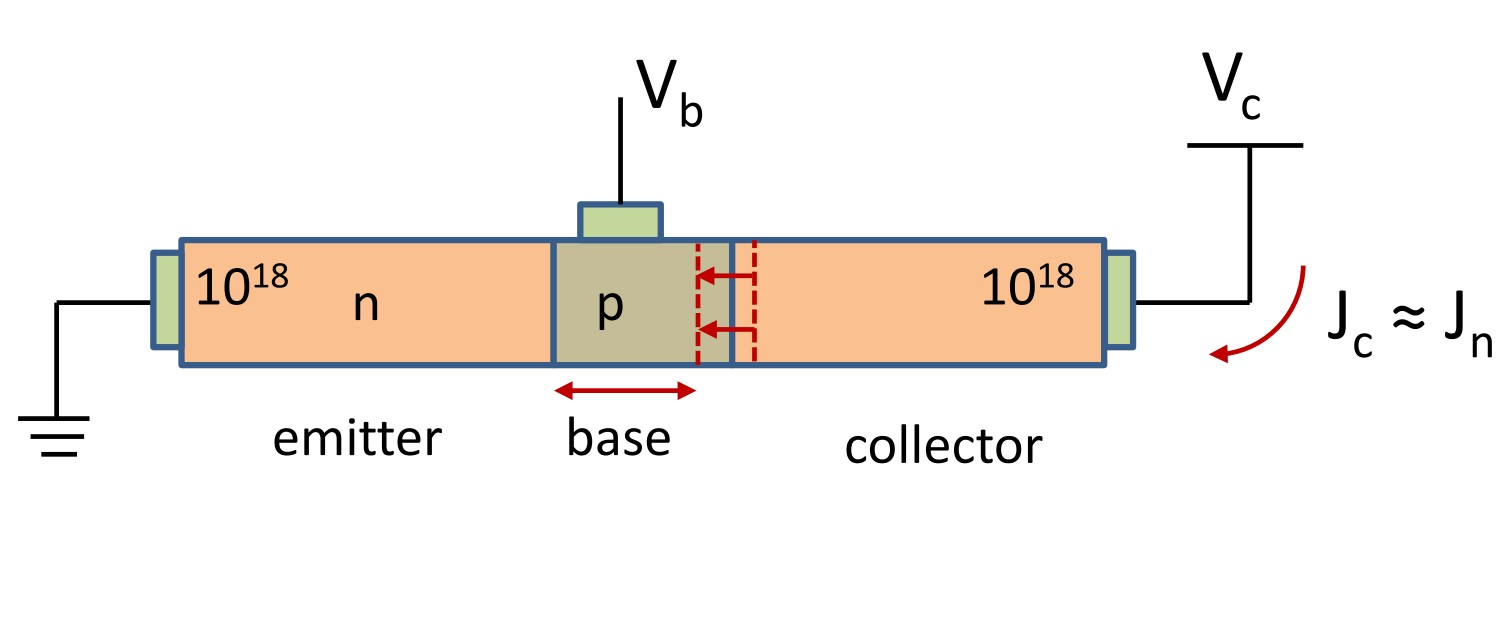
\includegraphics[width=0.8\linewidth]{BJT-two-pn.jpg}
    \end{figure}
    \begin{equation*}
        \begin{aligned}
            I_c = \beta I_s \left( \e^{\frac{eV_b}{nkT} } - 1 \right)
        \end{aligned}
    \end{equation*}
    Early Effects:
    \begin{figure}[H]
        \centering
        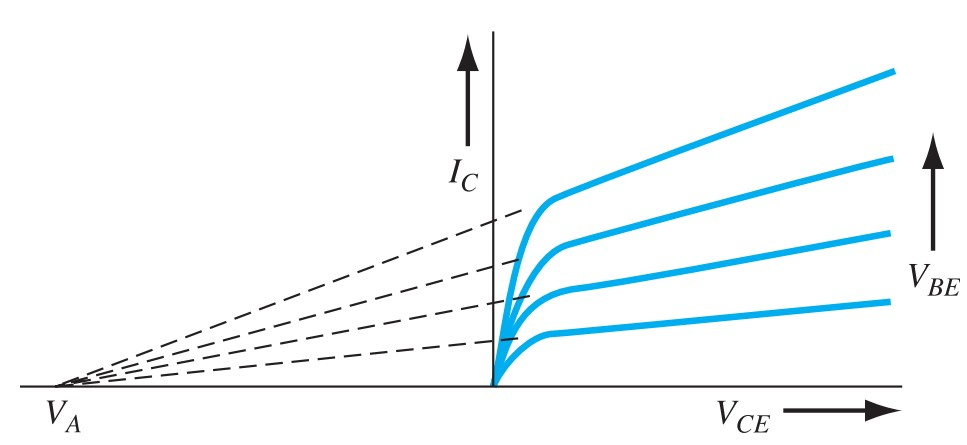
\includegraphics[width=0.8\linewidth]{Early-effect.jpg}
    \end{figure}
\end{document}